\documentclass{article}
\usepackage[top=2.5cm, left=3cm, right=3cm, bottom=4.0cm]{geometry}
\usepackage{graphicx} 
\usepackage{amsfonts,amsmath,amssymb}
\usepackage{array}
\usepackage{tabularray}
\usepackage[utf8]{inputenc}
\usepackage[T1]{fontenc}
\usepackage{csquotes}
\usepackage{alphabeta}
\usepackage{tabularx}
\usepackage{url}
\usepackage{hyperref}
\usepackage{esint}

\begin{document}
\begin{table}[ht]
    \begin{tblr}{
        @{}X[l, valign=b]X[c, valign=b]X[r, valign=b]@{}
    }

    \hline
    % First line, course info
    \SetCell[c=2]{l}{[ΘΠ04] Παράλληλα Συστήματα} & & {2024-25} \\ 
    \hline
    {} & {} & {} \\

    % Title
    \SetCell[c=3]{c}{ \Large \textbf{Εργασία 4 - Προγραμματισμός με CUDA} } \\
    {} & {} & {} \\

    % Name Surname, Student ID
    \hline
    \SetCell[c=3]{c}{ \textbf{Ονοματεπώνυμο:} Μάριος Γιαννόπουλος } \\
    \SetCell[c=3]{c}{ \textbf{A.M.:} 1115200000032} \\
    \hline

    \end{tblr}
\end{table}
\section{Εισαγωγή}
Η εργασία αυτή αφορά την επιτάχυνση ενός προγράμματος που υλοποιεί έναν επιλυτή Ν-σωμάτων (N-body simulator) χρησιμοποιώντας CUDA. Ο επιλυτής Ν-σωμάτων προσομοιώνει την κίνηση μιας ομάδας σωμάτων που αλληλεπιδρούν βαρυτικά μεταξύ τους. Η επιτάχυνση του προγράμματος επιτεύχθηκε με τη χρήση της πλατφόρμας CUDA, η οποία επιτρέπει την παράλληλη εκτέλεση υπολογισμών σε GPU.
\section{Περιγραφή Προβλήματος}
Το πρόβλημα που αντιμετωπίζουμε είναι ο υπολογισμός των βαρυτικών δυνάμεων μεταξύ Ν σωμάτων και η ενημέρωση των θέσεων τους σε κάθε χρονικό βήμα. Ο αρχικός κώδικας εκτελείται σε CPU και απαιτεί σημαντικό χρόνο για μεγάλο αριθμό σωμάτων. Συγκεκριμένα, για 4096 σώματα απαιτείται χρόνος εκτέλεσης περίπου 5 δευτερόλεπτα, ενώ για 65536 σώματα ο χρόνος εκτέλεσης φτάνει τα 20 λεπτά.
\section{Λύση}
Για την επιτάχυνση του προγράμματος, αναπτύχθηκαν δύο CUDA πυρήνες (kernels):
\begin{itemize}
    \item \texttt{bodyForceKernel}: Υπολογίζει τις βαρυτικές δυνάμεις που ασκούνται σε κάθε σώμα από όλα τα υπόλοιπα σώματα.
    \item \texttt{integratePositionKernel}: Ενημερώνει τις θέσεις των σωμάτων με βάση τις ταχύτητές τους.
\end{itemize}
Οι πυρήνες εκτελούνται παράλληλα στη GPU, με κάθε νήμα να αναλαμβάνει τον υπολογισμό για ένα σώμα. Η διαχείριση της μνήμης γίνεται με τη χρήση των συναρτήσεων \texttt{cudaMalloc} και \texttt{cudaMemcpy}, ενώ η συγχρονισμός των νημάτων εξασφαλίζεται με τη χρήση της \texttt{cudaDeviceSynchronize}.

\section{Αποτελέσματα}
Η επιτάχυνση του προγράμματος ήταν σημαντική. Τα αποτελέσματα για τους δύο βασικούς αριθμούς σωμάτων παρουσιάζονται στον παρακάτω πίνακα:

\begin{table}[h]
\centering
\begin{tabular}{|c|c|c|}
\hline
\textbf{Αριθμός Σωμάτων} & \textbf{Χρόνος Εκτέλεσης (s)} & \textbf{Αλληλεπιδράσεις/Δευτερόλεπτο (Billion)} \\
\begin{verbatim}
Running nbody simulator with 4096 bodies
----------------------------------------

Application should run faster than 0.9s
Your application ran in: 0.1424s
Your application reports  49.028 Billion Interactions / second

Your results are correct

Running nbody simulator with 65536 bodies
----------------------------------------

Application should run faster than 1.3s
Your application ran in: 0.2135s
Your application reports  416.817 Billion Interactions / second

Your results are correct
\end{verbatim}
% \hline
% 4096 & 0.1424 & 49.028 \\
% 65536 & 0.2135 & 416.817 \\
% \hline
\end{tabular}
\caption{Αποτελέσματα Επιτάχυνσης}
\end{table}

Όπως φαίνεται, ο χρόνος εκτέλεσης για 4096 σώματα μειώθηκε σε 0.1424 δευτερόλεπτα, ενώ για 65536 σώματα σε 0.2135 δευτερόλεπτα. Αυτό αντιστοιχεί σε 49.028 και 416.817 δισεκατομμύρια αλληλεπιδράσεις ανά δευτερόλεπτο, αντίστοιχα.

\section{Συμπεράσματα}
Η χρήση της CUDA για την επιτάχυνση του επιλυτή Ν-σωμάτων απέδωσε εξαιρετικά αποτελέσματα. Ο χρόνος εκτέλεσης μειώθηκε σημαντικά, περνώντας τα κριτήρια επιτυχίας της εργασίας. Η παράλληλη επεξεργασία στο GPU αποτελεί μια ισχυρή λύση για προβλήματα μεγάλης υπολογιστικής πολυπλοκότητας, όπως η προσομοίωση Ν-σωμάτων.

\section{Πηγαίος Κώδικας}
Ο πηγαίος κώδικας της εφαρμογής βρίσκεται στον φάκελο \texttt{src} του project. Περιλαμβάνει τα αρχεία:
\begin{itemize}
    \item \texttt{01-nbody.cu}: Ο κύριος κώδικας της εφαρμογής.
    \item \texttt{timer.h}: Βοηθητική βιβλιοθήκη για τη μέτρηση του χρόνου εκτέλεσης.
    \item \texttt{files.h}: Βοηθητική βιβλιοθήκη για την ανάγνωση και εγγραφή αρχείων.
\end{itemize}
\section{Πιστοποιητικό}
Παρακάτω παρουσιάζεται το πιστοποιητικό επιτυχημένης ολοκλήρωσης του online course:
\begin{figure}[h]
\centering
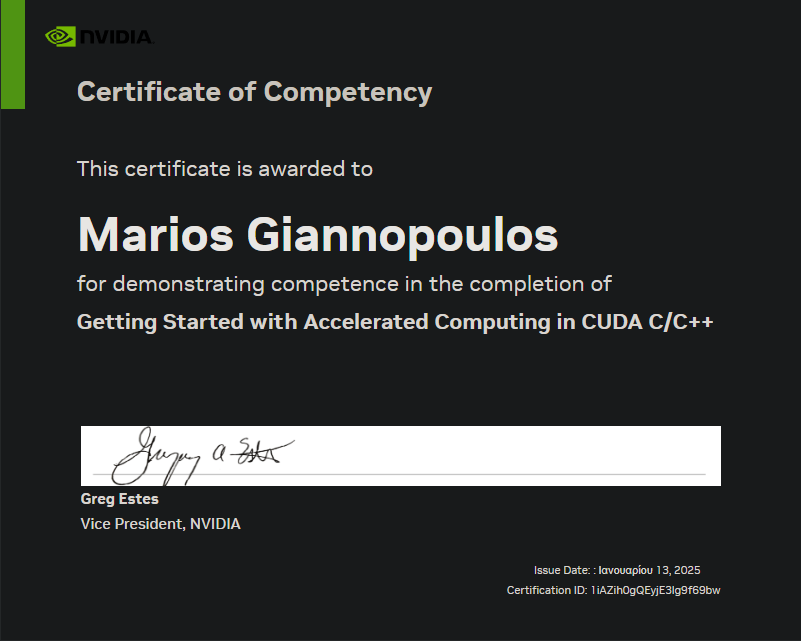
\includegraphics[width=0.8\textwidth]{certificate.png}
\caption{Πιστοποιητικό Ολοκλήρωσης}
\end{figure}
\end{document}